% Created by tikzDevice version 0.12.3.1 on 2021-06-19 00:10:43
% !TEX encoding = UTF-8 Unicode
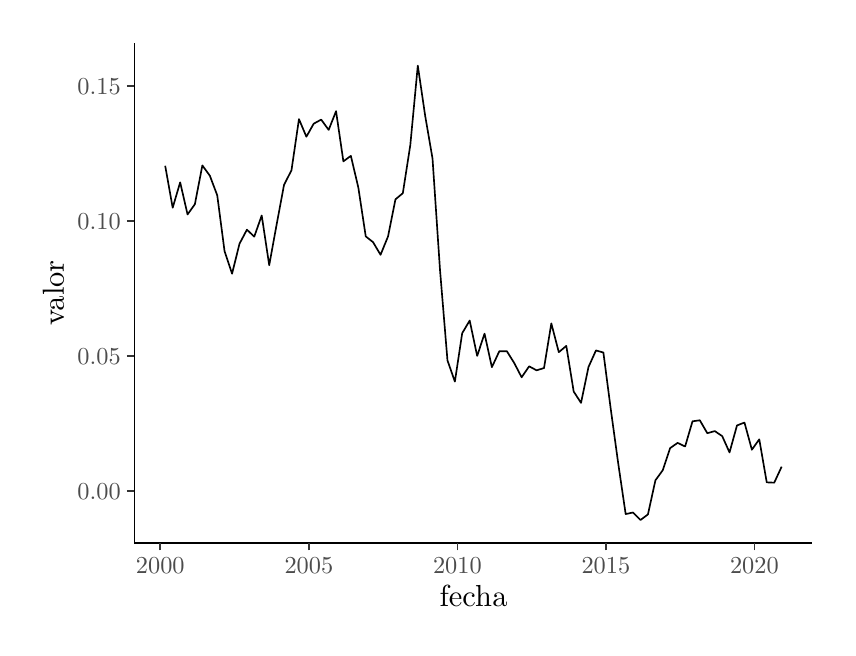
\begin{tikzpicture}[x=1pt,y=1pt]
\definecolor{fillColor}{RGB}{255,255,255}
\path[use as bounding box,fill=fillColor,fill opacity=0.00] (0,0) rectangle (289.08,216.81);
\begin{scope}
\path[clip] (  0.00,  0.00) rectangle (289.08,216.81);
\definecolor{drawColor}{RGB}{255,255,255}
\definecolor{fillColor}{RGB}{255,255,255}

\path[draw=drawColor,line width= 0.6pt,line join=round,line cap=round,fill=fillColor] (  0.00,  0.00) rectangle (289.08,216.81);
\end{scope}
\begin{scope}
\path[clip] ( 38.56, 30.69) rectangle (283.58,211.31);
\definecolor{fillColor}{RGB}{255,255,255}

\path[fill=fillColor] ( 38.56, 30.69) rectangle (283.58,211.31);
\definecolor{drawColor}{RGB}{0,0,0}

\path[draw=drawColor,line width= 0.6pt,line join=round] ( 49.69,166.90) --
	( 52.40,151.74) --
	( 55.10,160.92) --
	( 57.77,149.32) --
	( 60.42,153.01) --
	( 63.12,167.03) --
	( 65.83,163.31) --
	( 68.50,156.23) --
	( 71.14,136.06) --
	( 73.85,127.90) --
	( 76.55,138.75) --
	( 79.23,143.82) --
	( 81.87,141.28) --
	( 84.57,148.94) --
	( 87.28,130.98) --
	( 89.95,145.62) --
	( 92.63,159.98) --
	( 95.33,165.30) --
	( 98.03,183.77) --
	(100.71,177.40) --
	(103.35,182.11) --
	(106.06,183.59) --
	(108.76,179.87) --
	(111.43,186.62) --
	(114.08,168.51) --
	(116.78,170.49) --
	(119.49,158.99) --
	(122.16,141.39) --
	(124.80,139.30) --
	(127.51,134.74) --
	(130.21,141.36) --
	(132.89,154.76) --
	(135.56,157.00) --
	(138.26,174.37) --
	(140.97,203.10) --
	(143.64,184.93) --
	(146.29,169.53) --
	(148.99,129.34) --
	(151.69, 96.58) --
	(154.37, 88.91) --
	(157.01,106.40) --
	(159.72,110.98) --
	(162.42, 98.20) --
	(165.09,106.23) --
	(167.74, 94.13) --
	(170.44, 99.91) --
	(173.15, 99.90) --
	(175.82, 95.62) --
	(178.49, 90.48) --
	(181.20, 94.44) --
	(183.90, 92.99) --
	(186.58, 93.82) --
	(189.22,109.94) --
	(191.92, 99.54) --
	(194.63,101.82) --
	(197.30, 85.33) --
	(199.95, 81.23) --
	(202.65, 94.19) --
	(205.35,100.17) --
	(208.03, 99.43) --
	(210.67, 79.16) --
	(213.38, 59.42) --
	(216.08, 41.06) --
	(218.75, 41.61) --
	(221.43, 38.90) --
	(224.13, 40.92) --
	(226.83, 53.24) --
	(229.51, 56.93) --
	(232.15, 64.89) --
	(234.86, 66.77) --
	(237.56, 65.47) --
	(240.23, 74.56) --
	(242.88, 74.94) --
	(245.58, 70.27) --
	(248.29, 71.03) --
	(250.96, 69.23) --
	(253.61, 63.32) --
	(256.31, 73.07) --
	(259.01, 74.12) --
	(261.69, 64.31) --
	(264.36, 68.06) --
	(267.06, 52.51) --
	(269.77, 52.39) --
	(272.44, 58.17);
\end{scope}
\begin{scope}
\path[clip] (  0.00,  0.00) rectangle (289.08,216.81);
\definecolor{drawColor}{RGB}{0,0,0}

\path[draw=drawColor,line width= 0.6pt,line join=round] ( 38.56, 30.69) --
	( 38.56,211.31);
\end{scope}
\begin{scope}
\path[clip] (  0.00,  0.00) rectangle (289.08,216.81);
\definecolor{drawColor}{gray}{0.30}

\node[text=drawColor,anchor=base east,inner sep=0pt, outer sep=0pt, scale=  0.88] at ( 33.61, 46.45) {0.00};

\node[text=drawColor,anchor=base east,inner sep=0pt, outer sep=0pt, scale=  0.88] at ( 33.61, 95.16) {0.05};

\node[text=drawColor,anchor=base east,inner sep=0pt, outer sep=0pt, scale=  0.88] at ( 33.61,143.88) {0.10};

\node[text=drawColor,anchor=base east,inner sep=0pt, outer sep=0pt, scale=  0.88] at ( 33.61,192.60) {0.15};
\end{scope}
\begin{scope}
\path[clip] (  0.00,  0.00) rectangle (289.08,216.81);
\definecolor{drawColor}{gray}{0.20}

\path[draw=drawColor,line width= 0.6pt,line join=round] ( 35.81, 49.48) --
	( 38.56, 49.48);

\path[draw=drawColor,line width= 0.6pt,line join=round] ( 35.81, 98.19) --
	( 38.56, 98.19);

\path[draw=drawColor,line width= 0.6pt,line join=round] ( 35.81,146.91) --
	( 38.56,146.91);

\path[draw=drawColor,line width= 0.6pt,line join=round] ( 35.81,195.63) --
	( 38.56,195.63);
\end{scope}
\begin{scope}
\path[clip] (  0.00,  0.00) rectangle (289.08,216.81);
\definecolor{drawColor}{RGB}{0,0,0}

\path[draw=drawColor,line width= 0.6pt,line join=round] ( 38.56, 30.69) --
	(283.58, 30.69);
\end{scope}
\begin{scope}
\path[clip] (  0.00,  0.00) rectangle (289.08,216.81);
\definecolor{drawColor}{gray}{0.20}

\path[draw=drawColor,line width= 0.6pt,line join=round] ( 47.93, 27.94) --
	( 47.93, 30.69);

\path[draw=drawColor,line width= 0.6pt,line join=round] (101.62, 27.94) --
	(101.62, 30.69);

\path[draw=drawColor,line width= 0.6pt,line join=round] (155.28, 27.94) --
	(155.28, 30.69);

\path[draw=drawColor,line width= 0.6pt,line join=round] (208.94, 27.94) --
	(208.94, 30.69);

\path[draw=drawColor,line width= 0.6pt,line join=round] (262.60, 27.94) --
	(262.60, 30.69);
\end{scope}
\begin{scope}
\path[clip] (  0.00,  0.00) rectangle (289.08,216.81);
\definecolor{drawColor}{gray}{0.30}

\node[text=drawColor,anchor=base,inner sep=0pt, outer sep=0pt, scale=  0.88] at ( 47.93, 19.68) {2000};

\node[text=drawColor,anchor=base,inner sep=0pt, outer sep=0pt, scale=  0.88] at (101.62, 19.68) {2005};

\node[text=drawColor,anchor=base,inner sep=0pt, outer sep=0pt, scale=  0.88] at (155.28, 19.68) {2010};

\node[text=drawColor,anchor=base,inner sep=0pt, outer sep=0pt, scale=  0.88] at (208.94, 19.68) {2015};

\node[text=drawColor,anchor=base,inner sep=0pt, outer sep=0pt, scale=  0.88] at (262.60, 19.68) {2020};
\end{scope}
\begin{scope}
\path[clip] (  0.00,  0.00) rectangle (289.08,216.81);
\definecolor{drawColor}{RGB}{0,0,0}

\node[text=drawColor,anchor=base,inner sep=0pt, outer sep=0pt, scale=  1.10] at (161.07,  7.64) {fecha};
\end{scope}
\begin{scope}
\path[clip] (  0.00,  0.00) rectangle (289.08,216.81);
\definecolor{drawColor}{RGB}{0,0,0}

\node[text=drawColor,rotate= 90.00,anchor=base,inner sep=0pt, outer sep=0pt, scale=  1.10] at ( 13.08,121.00) {valor};
\end{scope}
\end{tikzpicture}
